% For a draft (single column, double spaced, line numbers):
\documentclass[review,12pt]{elsarticle}

% For a final (two column, single spaced):
% \documentclass[final,5p,times,twocolumn]{elsarticle}

\usepackage{xcolor}
\definecolor{ftbeige}{HTML}{FFF1E5} % Soft beige (FT-style)
\definecolor{softgray}{HTML}{EAEAEA} % Slightly darker light gray

\usepackage{geometry}
\makeatletter
\@ifclasswith{elsarticle}{review}{
    \geometry{margin=1in, top=1.2in, headheight=15pt}
    %\pagecolor{ftbeige}   % Toggle this for soft beige
    \pagecolor{softgray} % Toggle this for light gray
}{}
\makeatother
\usepackage{lineno}
 % (and \linenumbers after \end{frontmatter})
\renewcommand\linenumberfont{\normalfont\tiny\color{gray}}
\usepackage{amsmath,amssymb}
\usepackage{lipsum}
\usepackage{listings}
\usepackage{pgfplots}
\pgfplotsset{compat=1.18}
\usepackage[varqu]{inconsolata} % monospace font that is nicer than the default
\usepackage{tikz}
\usetikzlibrary{trees, positioning}
\usepackage{subcaption}

% --- DYNAMIC TRACKING HEADER CONFIGURATION ---
% Custom macro using native TeX registers (Guaranteed to compile on any system)
\newcount\scratchhour
\newcount\scratchminute

\newcommand{\compiledtimestamp}{%
  % Date formatting: YYYY-MM-DD
  \the\year-%
  \ifnum\month<10 0\fi\the\month-%
  \ifnum\day<10 0\fi\the\day~%
  % Calculate hours and minutes from total minutes since midnight (\time)
  \scratchhour=\time
  \divide\scratchhour by 60
  \scratchminute=\time
  \multiply\scratchhour by 60
  \advance\scratchminute by -\scratchhour
  \divide\scratchhour by 60
  % Time formatting: HH:MM hr
  \ifnum\scratchhour<10 0\fi\the\scratchhour:%
  %\ifnum\scratchminute<10 0\fi\the\scratchminute:%
  \ifnum\scratchminute<10 0\fi\the\scratchminute%
  %00~hr% Note: TeX engine primitives do not expose compilation seconds natively
  ~hr%
}

\usepackage{fancyhdr}
\pagestyle{fancy}
\fancyhf{} % Clear existing default headers/footers
\renewcommand{\headrulewidth}{0pt} % Remove the visual horizontal line under the header

% Inject the left-aligned custom tracking string ONLY for review/draft mode
\makeatletter
\@ifclasswith{elsarticle}{review}{
    \lhead{\footnotesize\ttfamily\color{gray}DRAFT - compiled \compiledtimestamp}
    \rhead{\thepage}
    
    % Force the fancy page style onto the first page/frontmatter layout
    \g@addto@macro\endfrontmatter{\thispagestyle{fancy}}
}{
    \pagestyle{plain}
}
\makeatother
% ------------------------------------------------

\lstdefinelanguage{Rust}{
  keywords={break, callback, continue, crate, else, enum, extern, false, fn, for, if, impl, in, let, loop, match, mod, move, mut, pub, ref, return, self, Self, static, struct, super, trait, true, type, unsafe, use, where, while, async, await, dyn, u8, u16, u32, u64, u128, i8, i16, i32, i64, i128, f32, f64, bool, char, str},
  otherkeywords={!, \&},
  sensitive=true,
  morecomment=[l]{//},
  morecomment=[s]{/*}{*/},
  morestring=[b]",
}

\usepackage{setspace}
\lstset{
  language=Rust,
  %basicstyle=\small\ttfamily,
  %basicstyle=\small\ttfamily\singlespacing,
  basicstyle=\small\ttfamily\setstretch{1.0}, % Adjust line spacing within code blocks
  numbers=left,
  numberstyle=\tiny\color{gray},
  stepnumber=1,
  numbersep=5pt,
  backgroundcolor=\color{white},
  showspaces=false,
  showstringspaces=false,
  showtabs=false,
  frame=single,
  rulecolor=\color{black},
  tabsize=4,
  captionpos=b,
  breaklines=true,
  breakatwhitespace=false,
  title=\lstname,
  keywordstyle=\color{blue},
  commentstyle=\color{gray},
  stringstyle=\color{red},
}

\journal{Journal to Be Determined}

\begin{document}

\begin{frontmatter}
\linenumbers

\title{Dualization-Based All-Hexahedral Mesh Generation: Algorithms and Performance Benchmarks}

\author{Michael R. Buche\corref{cor1}}
\ead{mrbuche@sandia.gov}
%\author{Chad B. Hovey}
\author{Chad B. Hovey}
\cortext[cor1]{Corresponding author}
\affiliation{organization={Sandia National Laboratories},
            city={Albuquerque NM}, country={United States of America}}
% \affiliation[b]{organization={Institute of Studies}, city={Sampleville}, country={Country}}

\begin{abstract}
This document demonstrates the two-column typeset (5p) layout produced by the
elsarticle class. It shows the Elsevier-style frontmatter, abstract, keywords,
sectioning, an equation, and a figure placeholder for visual evaluation.
\end{abstract}

%% Placeholder Outline
%\begin{verbatim}
%Existing Methods
%    Voxel start point (.npy | .spn) formats
%        Defeaturing (voxel end point)
%        Convert .npy to .spn
%        Convert .spn to .npy
%        (new!) Remesh .stl to .stl
%    Mesh start point (.exo | .inp | .mesh | .stl | .vtk)
%New Algorithms
%    Octree
%\end{verbatim}

\begin{keyword}
All-Hexahedral Mesh Generation \sep Octree Dualization \sep Finite Element Method \sep Rust Programming Language \sep Computational Geometry
\end{keyword}

\end{frontmatter}

\tableofcontents

\linenumbers

\section{Introduction}
\label{sec:intro}

\section{Methods}

\subsection{Input Geometry}

\subsubsection{Segmentation}

Let $n_x, n_y, n_z \in \mathbb{N}^+$ denote the number of voxels in each
coordinate direction.  The multi-index set
\begin{equation}
  \mathcal{I} = \{0,\ldots,n_x-1\}
              \times \{0,\ldots,n_y-1\}
              \times \{0,\ldots,n_z-1\}
\end{equation}
enumerates every voxel.  The indices $i$, $j$, $k$ are dimensionless natural
numbers; the voxel is the fundamental discrete unit of the 3D grid.  Given a scale
$(s_x, s_y, s_z) \in \mathbb{R}_{>0}^3$ (units: length~voxel$^{-1}$), the \emph{resolution}
\begin{equation}
  (\rho_x, \rho_y, \rho_z)
  = \left(\frac{1}{s_x},\, \frac{1}{s_y},\, \frac{1}{s_z}\right)
  \in \mathbb{R}_{>0}^3
\end{equation}
gives the number of voxels per unit length in each coordinate direction
(units: voxel~length$^{-1}$).  
In addition to the resolution, a translation $(t_x, t_y, t_z) \in \mathbb{R}^3$ (units: length) specifies the physical coordinates of the grid origin (the corner of voxel $(0,0,0)$).
Each voxel
$(i,j,k) \in \mathcal{I}$ occupies the axis-aligned rectangular region
\begin{equation}
  V_{ijk} = [i s_x + t_x,\; (i{+}1)s_x + t_x]
           \times [j s_y + t_y,\; (j{+}1)s_y + t_y]
           \times [k s_z + t_z,\; (k{+}1)s_z + t_z]
           \;\subset\; \mathbb{R}^3.
\end{equation}
The voxels tile the physical domain without overlap: the interiors of
$V_{ijk}$ and $V_{i'j'k'}$ are disjoint whenever $(i,j,k)\neq(i',j',k')$.
The total domain is therefore
\begin{equation}
  \Omega = \bigcup_{(i,j,k)\in\mathcal{I}} V_{ijk}
         = [t_x,\; n_x s_x + t_x]
           \times [t_y,\; n_y s_y + t_y]
           \times [t_z,\; n_z s_z + t_z].
\end{equation}

A \emph{segmentation} assigns to each voxel a material block identifier
via the label function
\begin{equation}
  \sigma : \mathcal{I} \to \mathcal{B},
\end{equation}
where $\mathcal{B} \subset \mathbb{N}_0$ is a finite set of block identifiers.
Block identifiers are non-negative integers, with a reserved sentinel value
denoting exterior or padding regions that do not correspond to a physical material.
The region associated with a given block $b$ is
\begin{equation}
  \Omega_b = \bigcup_{\substack{(i,j,k)\in\mathcal{I}\\\sigma(i,j,k)=b}} V_{ijk}.
\end{equation}
A user-specified removal set $\mathcal{R} \subseteq \mathcal{B}$
designates blocks to exclude from meshing, leaving the active domain
\begin{equation}
  \Omega^* = \bigcup_{\substack{(i,j,k)\in\mathcal{I}\\\sigma(i,j,k)\notin\mathcal{R}}} V_{ijk}.
\end{equation}

\subsubsection{Tessellation}

A tessellation is a piecewise-linear approximation of a surface
$\Gamma \subset \mathbb{R}^3$, typically the boundary of a body to be meshed.
It is defined by a vertex set
\begin{equation}
  \mathcal{V} = \bigl\{\mathbf{x}_p \in \mathbb{R}^3 : p = 0,\ldots,N_v - 1\bigr\}
\end{equation}
of $N_v$ points, together with a face set of $N_f$ triangles.  Each face
$t \in \{0,\ldots,N_f-1\}$ is identified by a connectivity triple
$(p_0^t,\, p_1^t,\, p_2^t) \in \{0,\ldots,N_v-1\}^3$ and defines the
planar triangle
\begin{equation}
  T_t = \operatorname{conv}\bigl\{
    \mathbf{x}_{p_0^t},\, \mathbf{x}_{p_1^t},\, \mathbf{x}_{p_2^t}
  \bigr\} \subset \mathbb{R}^3,
\end{equation}
where $\operatorname{conv}$ denotes the convex hull --- the smallest convex
set containing the three vertices.  Equivalently, using barycentric
coordinates,
\begin{equation}
  T_t = \Bigl\{
    \alpha_0\,\mathbf{x}_{p_0^t}
    + \alpha_1\,\mathbf{x}_{p_1^t}
    + \alpha_2\,\mathbf{x}_{p_2^t}
    \;\Big|\;
    \alpha_i \geq 0,\; \alpha_0 + \alpha_1 + \alpha_2 = 1
  \Bigr\} \subset \mathbb{R}^3.
\end{equation}
The tessellated surface is the union of all triangles,
\begin{equation}
  \Gamma_h = \bigcup_{t=0}^{N_f-1} T_t,
\end{equation}
which serves as a piecewise-linear approximation of $\Gamma$.
Each triangle carries a unit outward normal
\begin{equation}
  \hat{\mathbf{n}}_t =
    \frac{
      (\mathbf{x}_{p_1^t} - \mathbf{x}_{p_0^t})
      \times
      (\mathbf{x}_{p_2^t} - \mathbf{x}_{p_0^t})
    }{
      \bigl\|
        (\mathbf{x}_{p_1^t} - \mathbf{x}_{p_0^t})
        \times
        (\mathbf{x}_{p_2^t} - \mathbf{x}_{p_0^t})
      \bigr\|
    } \in S^2,
\end{equation}
where $S^2$ denotes the unit sphere in $\mathbb{R}^3$.
Tessellations are read from and written to STL files, in which all
vertex coordinates and normal components are stored as \lstinline!f32!
(IEEE~754 single-precision floating-point).

\subsection{Octree}

The octree is generated from a singleton, level zero cell that is an axis-aligned bounding box of the input geometry, which can be a segmentation or tessellation.

The level zero cell is subsequently subdivided into eight children cells based on a criterion, such as the presence of geometry within the cell itself, or a maximum depth limit.

A \emph{cell} is defined as a recursive spatial partition of an axis-aligned bounding volume. Each cell $C$ is encoded by a grid origin $(m_x, m_y, m_z) \in \mathbb{N}_0^3$ and a grid edge length $\ell \in \{1, 2, 4, \ldots, n\}$, where $n$ is the root edge length (a power of two). The same length $\ell$ applies in all three coordinate directions, so every cell is a cube in integer grid space; cells at deeper levels of the tree have smaller $\ell$, with $\ell = 1$ identifying the finest-resolution leaf cells (termed \emph{voxel cells} in the implementation). Given a scale $(s_x, s_y, s_z) \in \mathbb{R}_{>0}^3$ and translation $(t_x, t_y, t_z) \in \mathbb{R}^3$, the physical region occupied by $C$ is
\begin{equation}
  \Omega_C = [m_x s_x + t_x,\; (m_x{+}\ell)\,s_x + t_x]
           \times [m_y s_y + t_y,\; (m_y{+}\ell)\,s_y + t_y]
           \times [m_z s_z + t_z,\; (m_z{+}\ell)\,s_z + t_z]
           \subset \mathbb{R}^3,
\end{equation}
with physical dimensions $\ell s_x \times \ell s_y \times \ell s_z$.  When the scale is isotropic, $s_x = s_y = s_z = s$, the physical cell is also a cube with side length $\ell s$; this is always the case for tessellation-based octrees, where the scale is set uniformly from the minimum cell size.  For segmentation-based octrees, an anisotropic scale (differing voxel dimensions in $x$, $y$, $z$) produces rectangular cuboid cells in physical space.

A cell is either:

\begin{itemize}
  \item A \textbf{leaf cell}, representing a terminal node in the tree that holds a block identifier $b(C) \in \{0,\ldots,254\}$, with 255 reserved as a padding sentinel for exterior cells, or
  \item A \textbf{non-leaf cell}, which has been subdivided into eight equal-sized child octants (or four quadrants in 2D).
\end{itemize}

A non-leaf cell $C$ with edge length $\ell$ is subdivided into eight children $\{C_{ijk}\}_{(i,j,k)\in\{0,1\}^3}$, where child $C_{ijk}$ has grid origin $(m_x + i\ell/2,\; m_y + j\ell/2,\; m_z + k\ell/2)$ and edge length $\ell/2$. The children tile the parent exactly,
\begin{equation}
  \Omega_C = \bigcup_{(i,j,k)\,\in\,\{0,1\}^3} \Omega_{C_{ijk}},
  \qquad
  \operatorname{int}(\Omega_{C_{ijk}}) \cap \operatorname{int}(\Omega_{C_{i'j'k'}}) = \emptyset
  \quad (i,j,k) \neq (i',j',k').
\end{equation}
Denoting the set of leaf cells of the octree $\mathcal{T}$ by $\mathcal{L}(\mathcal{T})$, the leaf cells partition the root domain $\Omega_0 = \Omega_{C_0}$,
\begin{equation}
  \Omega_0 = \bigcup_{C\,\in\,\mathcal{L}(\mathcal{T})} \Omega_C,
  \qquad
  \operatorname{int}(\Omega_C) \cap \operatorname{int}(\Omega_{C'}) = \emptyset
  \quad C \neq C'.
\end{equation}
For a segmentation input, a cell is assigned block $b$ if all voxels within its grid region share label $b$ (i.e., $\sigma(i,j,k) = b$ for all $(i,j,k) \in \mathcal{I}$ contained in $\Omega_C$); otherwise it is subdivided. For a tessellation input, a cell is subdivided if it contains surface samples (vertices of $\Gamma_h$) and has edge length $\ell > 1$; otherwise it is assigned a uniform block.

\subsubsection{Quadtree Illustration}

A quadtree is a 2D analog of an octree, where each cell is subdivided into four quadrants instead of eight octants. Fig.~\ref{fig:quadtree_hierarchy} shows an example quadtree structure.

\begin{figure}[htbp]
    \centering
    % Part A: Spatial Decomposition
    \begin{subfigure}{0.45\textwidth}
        \centering
        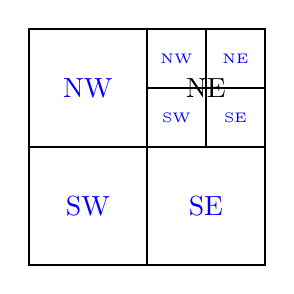
\begin{tikzpicture}[scale=3, thick]
            % Level 0
            \draw (0,0) rectangle (1,1);
            
            % Level 1
            \draw (0.5,0) -- (0.5,1);
            \draw (0,0.5) -- (1,0.5);
            
            % Level 2 (Subdivision of Northeast quadrant)
            \begin{scope}[shift={(0.5,0.5)}, scale=0.5]
                \draw (0.5,0) -- (0.5,1);
                \draw (0,0.5) -- (1,0.5);
                \node[blue] at (0.25, 0.25) {\tiny SW};
                \node[blue] at (0.75, 0.25) {\tiny SE};
                \node[blue] at (0.25, 0.75) {\tiny NW};
                \node[blue] at (0.75, 0.75) {\tiny NE};
            \end{scope}
            
            % Level 1 Labels
            \node[blue] at (0.25, 0.25) {SW};
            \node[blue] at (0.75, 0.25) {SE};
            \node[blue] at (0.25, 0.75) {NW};
            \node at (0.75, 0.75) {NE};
        \end{tikzpicture}
        \caption{Spatial Decomposition}
    \end{subfigure}
    \hfill
    % Part B: Tree Hierarchy (Inverted Tree)
    \begin{subfigure}{0.45\textwidth}
        \centering
        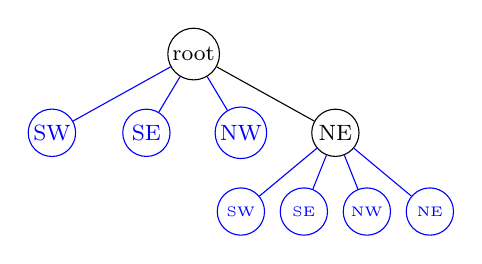
\begin{tikzpicture}[
            level 1/.style={sibling distance=12mm, level distance=10mm},
            level 2/.style={sibling distance=8mm, level distance=10mm, blue},
            every node/.style={circle, draw, minimum size=6mm, inner sep=1pt, font=\footnotesize}
        ]
            \node {root}
                child[blue] { node {SW} }
                child[blue] { node {SE} }
                child[blue] { node {NW} }
                child { node {NE}
                    child { node {\tiny SW} }
                    child { node {\tiny SE} }
                    child { node {\tiny NW} }
                    child { node {\tiny NE} }
                };
        \end{tikzpicture}
        \caption{Tree Hierarchy}
    \end{subfigure}
    \caption{(a)~A quadtree decomposition showing two levels of refinement.  The first level of refinement (level~0 to level~1), shows decomposition in the the SW, SE, NW, and NE children.  The second level of refinement (level~1 to level~2), shows decomposition of the level 1 NE cell into four children. (b)~The quadtree illustrated as an inverted tree hierarchy.  Leaf cells are in blue, non-leaf cells are in black.}
    \label{fig:quadtree_hierarchy}
\end{figure}

\subsubsection{Cell Data Structure}

The implementation represents each octree cell using the \texttt{Cell} structure shown in Listing~\ref{lst:cell_struct}. This structure encodes the cell's spatial domain through its origin (\texttt{min\_x}, \texttt{min\_y}, \texttt{min\_z}) and edge length (\texttt{lngth}), utilizing \texttt{u16} integer grid units for memory efficiency. Hierarchical relationships are maintained via \texttt{cells}, which stores indices to eight children for subdivided nodes, while topological connectivity is captured by \texttt{faces}, referencing the indices of six neighboring cells. An optional \texttt{block} field identifies the material assignment for leaf cells.


\begin{lstlisting}[language=Rust, caption={Rust implementation of the octree cell structure.}, label={lst:cell_struct}]
// src/tree/mod.rs
pub struct Cell {
    pub block: Option<u8>,   // Optional material or block ID
    cells: Option<Indices>,  // Indices to 8 children, if subdivided
    faces: Faces,            // Indices to 6 neighbor cells
    lngth: u16,              // Edge length (Grid units)
    min_x: u16,              // origin x coordinate (Grid units)
    min_y: u16,              // origin y coordinate (Grid units)
    min_z: u16,              // origin z coordinate (Grid units)
}
\end{lstlisting}

\begin{itemize}
\item Coordinate Precision: The use of u16 for spatial data (\texttt{min\_x}, \texttt{min\_y}, \texttt{min\_z}) supports up to $2^{16} = 65,536$ discrete grid step units in each dimension.  The memory overhead per spatial field is 16 bits, compared to 32 or 64 bits for floating-point representations. This allows for efficient storage and fast computations while maintaining sufficient precision for the grid-based representation of the octree.
\item Neighbor Storage: The \lstinline!Faces! array stores \lstinline!Option<usize>! indices to the six face-adjacent neighbor cells. The local face numbering convention is: 0 ($-y$), 1 ($+x$), 2 ($+y$), 3 ($-x$), 4 ($-z$), and 5 ($+z$). In the case where the domain boundary occurs (no neighbor can ever exist), \lstinline!None! is used. \lstinline!None! is also used as a transient construction state, where the interior face has not yet been paired during tree construction (e.g., freshly subdivided siblings before the \lstinline!subdivide()! function wires up adjacency).
\end{itemize}

\subsubsection{Memory Efficiency}

A key aspect of the implementation is the use of the \lstinline!u16! type for the cell's minimum coordinates (\lstinline!min_x!, \lstinline!min_y!, \lstinline!min_z!) and length (\lstinline!lngth!) instead of a typical \lstinline!f64! or \lstinline!f32! floating-point type. This design choice allows for efficient storage and fast computations while maintaining sufficient precision for the grid-based representation of the octree. 

The memory requirement $M$ (in MB) is calculated as $M = N \times S / 10^6$, where $N$ is the number of cells and $S$ is the size of a single cell in bytes. On a 64-bit system, the actual size of the \lstinline!Cell! struct (verifiable via Rust's \lstinline!std::mem::size_of::<Cell>()!) is $S \approx 184$~bytes. The field-by-field breakdown, listed from small to large, is as follows:

\begin{itemize}
  \item \lstinline!block! (\lstinline!Option<u8>!): 2~bytes (1~byte discriminant + 1~byte value).
  \item Struct alignment padding: 6~bytes (to round the total to the struct's 8-byte alignment).
  \item Spatial data (4 $\times$ \lstinline!u16!: \lstinline!min_x!, \lstinline!min_y!, \lstinline!min_z!, \lstinline!lngth!): $4 \times 2 = 8$~bytes.
  \item \lstinline!cells! (\lstinline!Option<[usize; 8]>!): 72~bytes (1~byte discriminant + 7~bytes alignment padding + $8 \times 8 = 64$~bytes of child indices).
  \item \lstinline!faces! (\lstinline![Option<usize>; 6]!): 96~bytes ($6 \times 16$~bytes, where each \lstinline!Option<usize>! requires 1~byte discriminant + 7~bytes alignment padding + 8~bytes value, since \lstinline!usize! has no niche and cannot use Rust's null-pointer optimization).
\end{itemize}

In contrast, if the spatial data were stored as \lstinline!f64!, only the four spatial fields grow: from $4 \times 2 = 8$~bytes to $4 \times 8 = 32$~bytes, yielding $S \approx 208$~bytes. All other fields---\lstinline!block!, \lstinline!cells!, and \lstinline!faces!---remain identical in size, since they store integer indices regardless of the spatial representation. The \lstinline!u16! approach therefore reduces memory by 24~bytes per cell, an approximately 11.5\% reduction, as illustrated in Figure~\ref{fig:memory_req}. Notably, the \lstinline!cells! and \lstinline!faces! index fields together account for 168 of the 184~bytes (91\%), making them the dominant contributor to the per-cell footprint.


Figure~\ref{fig:memory_req} illustrates the memory requirement as a function of octree size, comparing the \lstinline!u16! approach with a standard \lstinline!f64! approach.

\begin{figure}[h]
\centering
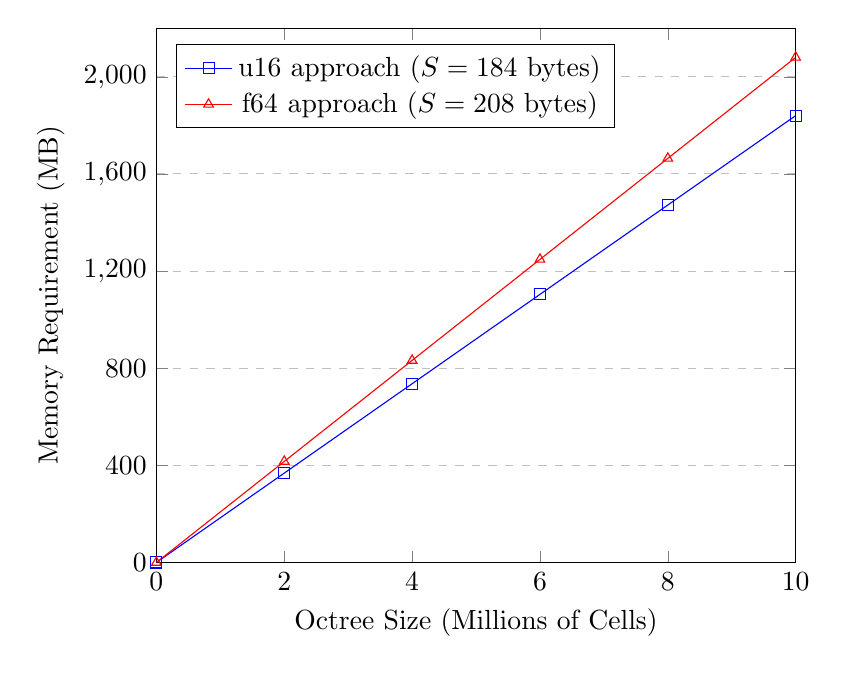
\begin{tikzpicture}
\begin{axis}[
    xlabel={Octree Size (Millions of Cells)},
    ylabel={Memory Requirement (MB)},
    xmin=0, xmax=10,
    ymin=0, ymax=2200,
    xtick={0,2,4,6,8,10},
    ytick={0,400,800,1200,1600,2000},
    legend pos=north west,
    ymajorgrids=true,
    grid style=dashed,
    width=0.8\columnwidth
]

\addplot[
    color=blue,
    mark=square,
    ]
    coordinates {
    (0,0)(2,368)(4,736)(6,1104)(8,1472)(10,1840)
    };
    \addlegendentry{\lstinline!u16! approach ($S = 184$~bytes)}

\addplot[
    color=red,
    mark=triangle,
    ]
    coordinates {
    (0,0)(2,416)(4,832)(6,1248)(8,1664)(10,2080)
    };
    \addlegendentry{\lstinline!f64! approach ($S = 208$~bytes)}

\end{axis}
\end{tikzpicture}
\caption{Memory requirement comparison between \lstinline!u16! ($S = 184$~bytes) and \lstinline!f64! ($S = 208$~bytes) cell representations. The difference of 24~bytes per cell reflects the cost of the four spatial coordinate fields only; index fields (\lstinline!cells! and \lstinline!faces!) are identical in both cases.}
\label{fig:memory_req}
\end{figure}

\subsubsection{Normalized Grid Initialization}
When an octree is constructed from a surface (see \texttt{src/tree/tessellation/mod.rs}) the physical coordinates from the STL input are transformed into a normalized integer space.
The \lstinline!scale! and \lstinline!translation! are stored in the \lstinline!Octree! \lstinline!struct!, and the
samples are shifted such that they fit into a grid defined by \lstinline!u16! indices.

\subsubsection{Robust Node Matching via \lstinline!NodeMap!}
An important decision was made on how to robustly handle nodes that exist in the dualized
space. These dual nodes exist at cell centers, face centers, or edge centers. 
Since they fall on ``half-grid'' locations, they cannot be directly indexed using the \lstinline!u16! grid coordinates. To address this, our data structure uses a \lstinline!NodeMap! with integer keys scaled by 2:

\begin{lstlisting}[language=Rust, caption={Rust implementation using the \lstinline!NodeMap! with integer keys scaled by 2.}, label={lst:node_map_scale_2}]
// src/tree/mod.rs
type NodeMap = HashMap<[usize; NSD], usize>;

// src/tree/hex/edge_template_1/mod.rs
nodes_map.insert(
    [
        (2.0 * nodal_coordinates[...][0]) as usize,
        (2.0 * nodal_coordinates[...][1]) as usize,
        (2.0 * nodal_coordinates[...][2]) as usize,
    ],
    node_index
)
\end{lstlisting}

By mutiplying the coordinates (which are often half-integers like \lstinline!x.5!) by 2.0 and casting to a \lstinline!usize!, we create a perfect integer hash key that uniquely identifies each node in the dual space. In contrast, an approach using \lstinline!f64! keys would require careful handling of floating-point precision issues, and a \lstinline!u16! key approach would not be able to represent the half-integer positions accurately. This method ensures robust node matching without the pitfalls of floating-point comparisons or the limitations of integer indexing.

\subsubsection{Late-Stage Physical Transformation}
Physical \lstinline!f64! coordinates are only generated at the very last step during the conversion to a \lstinline!FiniteElementMesh!:

\begin{lstlisting}[language=Rust, caption={Late-stage physical transformation of node coordinates.}, label={lst:late_stage_transform}]
// src/tree/hex/mod.rs
let nodal_coordinates = coordinates_0
    .iter()
    .map(|coordinate| {
        [
            coordinate[0] * tree.scale.x() + tree.translate.x(),
            coordinate[1] * tree.scale.y() + tree.translate.y(),
            coordinate[2] * tree.scale.z() + tree.translate.z(),
        ].into()
    })
    .collect();
\end{lstlisting}

Integer arithmetic and integer-based \lstinline!HashMap! lookups are generally faster than their floating-point counterparts. By deferring the conversion to physical \lstinline!f64! coordinates until the final stage, we can perform all intermediate computations using the more efficient integer representation.

In addition to efficiency, this approach also enhances robustness. By avoiding floating-point arithmetic during the octree construction and dualization processes, we eliminate potential issues related to floating-point precision and rounding errors.

\section{Conclusion}
%\lipsum[4]
%
%\begin{figure}[t]
%\centering
%\framebox[0.9\columnwidth][c]{\rule{0pt}{3cm}\textit{Figure placeholder}}
%\caption{A single-column figure spanning one column width.}
%\label{fig:sample}
%\end{figure}


\end{document}
